\documentclass{article}
\usepackage{graphicx}
\usepackage[a4paper, hmargin = 2.5cm, vmargin = 2.5cm]{geometry}
\usepackage[english]{babel}

\title{Database project: Travel agency \\ (Milestone 2)}
\author{Oliver Baltisberger, Rachid Flueckiger, Christian Pernet}
\date{\today}

\begin{document}
	\maketitle
	
	\section*{Adjustment of ER-Diagram}
	Based on the feedback that we received for Milestone 1, we slightly adjusted our ER-Diagram:
	\begin{itemize}
		\item The entity Payment is no longer modeled as a weak entity. Further, we allow installment payments (i.e. a client can pay for his individualized trip with several payments), which leads to a 1:N relationship.
		This also implies that the amount of the payment can be different from the price of the trip.
		\item We added the attributes City, Country and Date to the entity Activity. This allows us to know where and when an activity takes place.
		For simplicity reasons, we decided to drop the attribute Contact from the entity Activity. The phone number of the activity provider is not essential in our simplified model.
	\end{itemize}
	
You find our adjusted ER-Diagram on the next page.
	\newpage
	
	\section*{ER-Diagram}
	\begin{figure}[htbp]
		\centering
			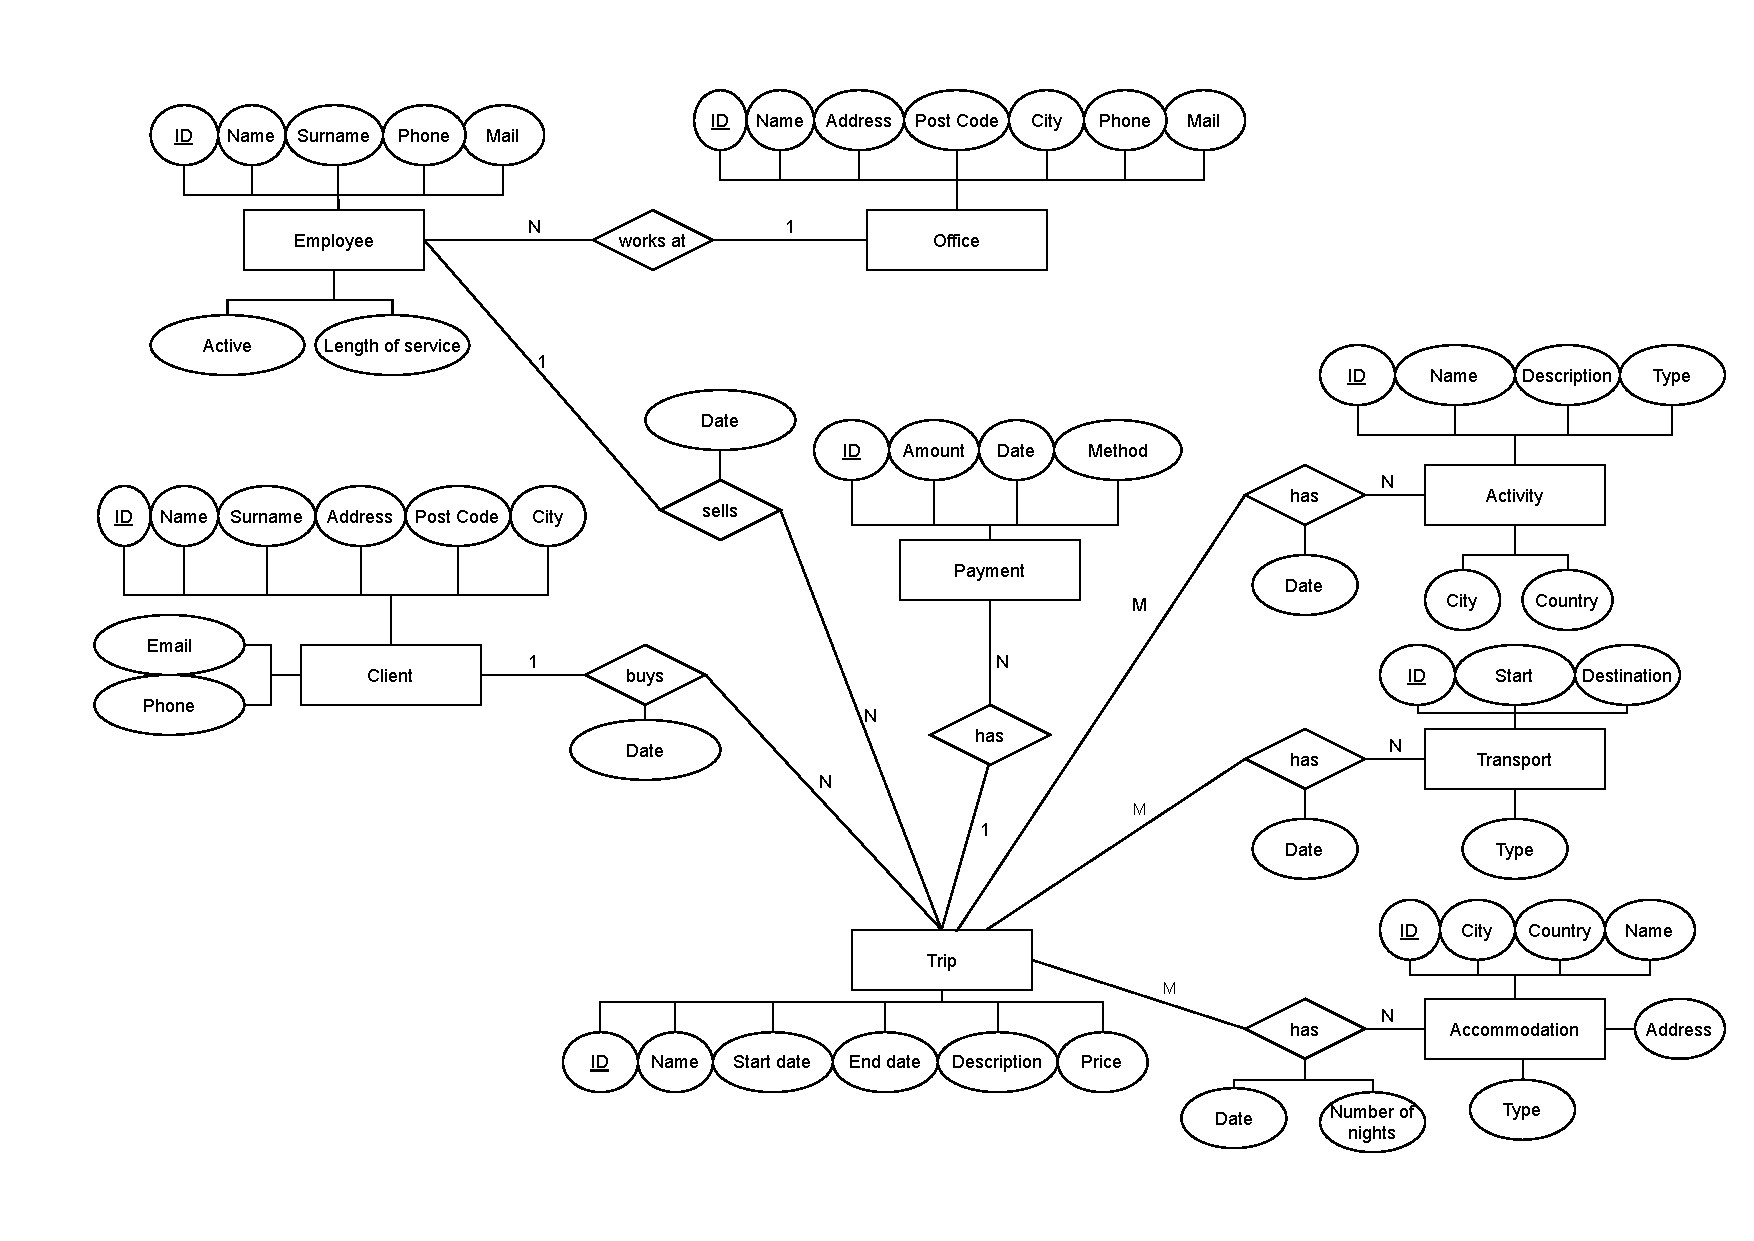
\includegraphics[width=1.15\textwidth, angle=90]{../Diagramm.pdf}
		\label{ER-Model}
		\caption{Travel agency ER-Diagram}
	\end{figure}
	

\end{document}